% This is a basic Math Paper

\documentclass[11pt]{article}

% Preamble

\usepackage[margin=1in]{geometry}
\usepackage{amsfonts, amsmath, amssymb}
\usepackage{fancyhdr, float, graphicx}
\usepackage[utf8]{inputenc} % Required for inputting international characters
\usepackage[T1]{fontenc} % Output font encoding for international characters
\usepackage{fouriernc} % Use the New Century Schoolbook font
\usepackage[nottoc, notlot, notlof]{tocbibind}
\usepackage{url}
%\usepackage{minted}
\usepackage{listings}
\usepackage{color}

\lstset{frame=tb,
	language=C++,
	aboveskip=3mm,
	belowskip=3mm,
	showstringspaces=false,
	columns=flexible,
	basicstyle={\small\ttfamily},
	numbers=none,
	numberstyle=\tiny\color{gray},
	keywordstyle=\color{blue},
	commentstyle=\color{dkgreen},
	stringstyle=\color{mauve},
	breaklines=true,
	breakatwhitespace=true,
	tabsize=4
}


\definecolor{dkgreen}{rgb}{0,0.6,0}
\definecolor{gray}{rgb}{0.5,0.5,0.5}
\definecolor{mauve}{rgb}{0.58,0,0.82}


% Header and Footer
\pagestyle{fancy}
\fancyhead{}
\fancyfoot{}
\fancyhead[L]{\textit{\Large{Working of Turbines}}}
%\fancyhead[R]{\textit{something}}
\fancyfoot[C]{\thepage}
\renewcommand{\footrulewidth}{1pt}


 
% Other Doc Editing
% \parindent 0ex
%\renewcommand{\baselinestretch}{1.5}

\begin{document}
	
	\begin{titlepage} 
		\centering 
		
		%---------------------------NAMES-------------------------------
%		\begin{figure}
%			\centering
%			
\includegraphics[scale=0.5]{logo.png}
%		\end{figure}

		\Huge\textsc{
			MIT World Peace University
		}\\

		\vspace{1.00\baselineskip} % space after Uni Name
		
		\LARGE{
			Basics of Electronics and Electrical Engineering\\
			ECE1022A, School of ECE\\
			First Year B. Tech, Trimester 2\\
			Academic Session 2021-22
		}
		
		\vfill % space after Sub Name

		
		%--------------------------TITLE-------------------------------
		
		\rule{\textwidth}{1.6pt}\vspace*{-\baselineskip}\vspace*{2pt}
		\rule{\textwidth}{0.6pt}
		\vspace{0.75\baselineskip} % Whitespace above the title
		
		
		
		\Huge{\textsc{
				8 Bit Mp3 Player
			}} \\
		
		
		
		\vspace{0.5\baselineskip} % Whitespace below the title
		\rule{\textwidth}{0.6pt}\vspace*{-\baselineskip}\vspace*{2.8pt}
		\rule{\textwidth}{1.6pt}
		
		\vspace{1\baselineskip} % Whitespace after the title block

		%--------------------------SUBTITLE --------------------------	
			
		\LARGE\textsc{
			Project Report\\
			For Project Based Learning Activity
		} % Subtitle or further description
		\vfill
		
		%--------------------------AUTHOR-------------------------------
		
		Prepared By
		\vspace{0.5\baselineskip} % Whitespace before the editors
		
		\Large{
			Krishnaraj Thadesar \\
			Division 9,
			Roll. 109054  (I3)\\
			PRN. 1032210888
		}
		
		
		\vspace{1\baselineskip} % Whitespace below the editor list
		\today

	\end{titlepage}
	
	
% Contents

\tableofcontents
\thispagestyle{empty}
\clearpage


\setcounter{page}{1}

% PAGE 1

\section{Introduction}
An Mp3 Player is a device that has only one purpose, which is to play Mp3 files or songs. It can sometimes include a Display to let you know which song is being played, and what the next songs are.\\

8 Bit Music got its name from Music generated from \textit{PSG(programmable Sound
Generator)} Chip, located usually on 8-bit Microprocessors as opposed to Modern 64 Bit ones. It uses limited Frequencies to create any sound or tune.\\

In This project we will use \textbf{Arduino UNO} which uses an \textbf{ATMega328} chipset, which is an \textit{8 Bit processor} combined with an LCD Screen to make a very simple Music Player.

\section{Circuit Diagram}
\subsection{Schematic Diagram}
\begin{figure}[H]
	\centering
	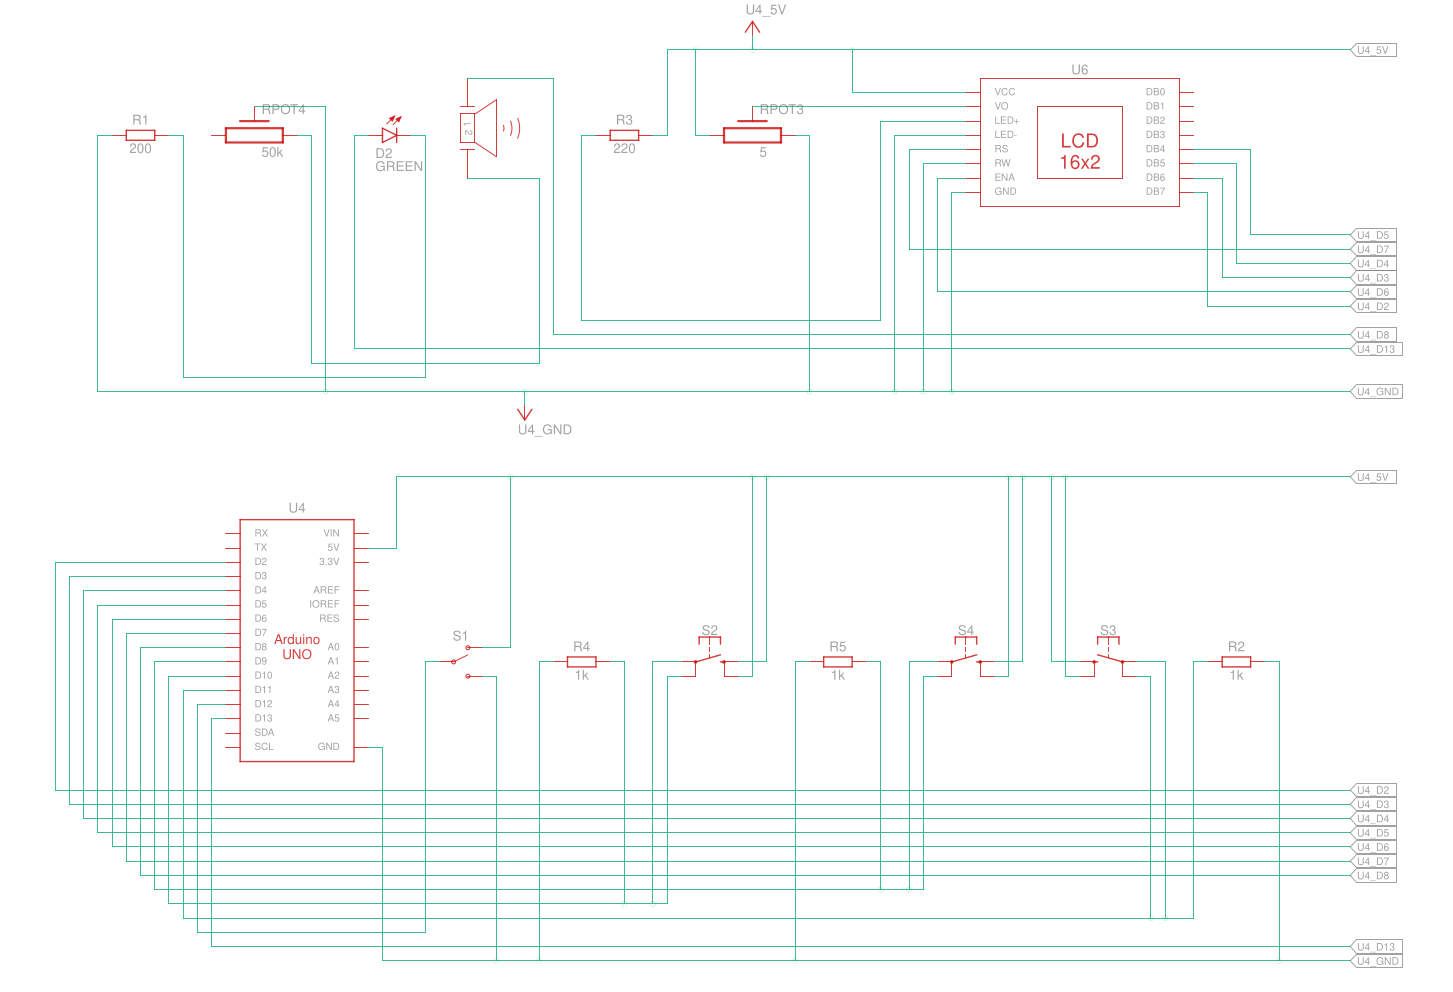
\includegraphics[scale=.45]{Main Circuit Diagram.png}
	\caption{Schematic Diagram}
	\label{fig:Schematic Diagram}
\end{figure}

\subsection{Simulation}
\begin{figure}[H]
	\centering
	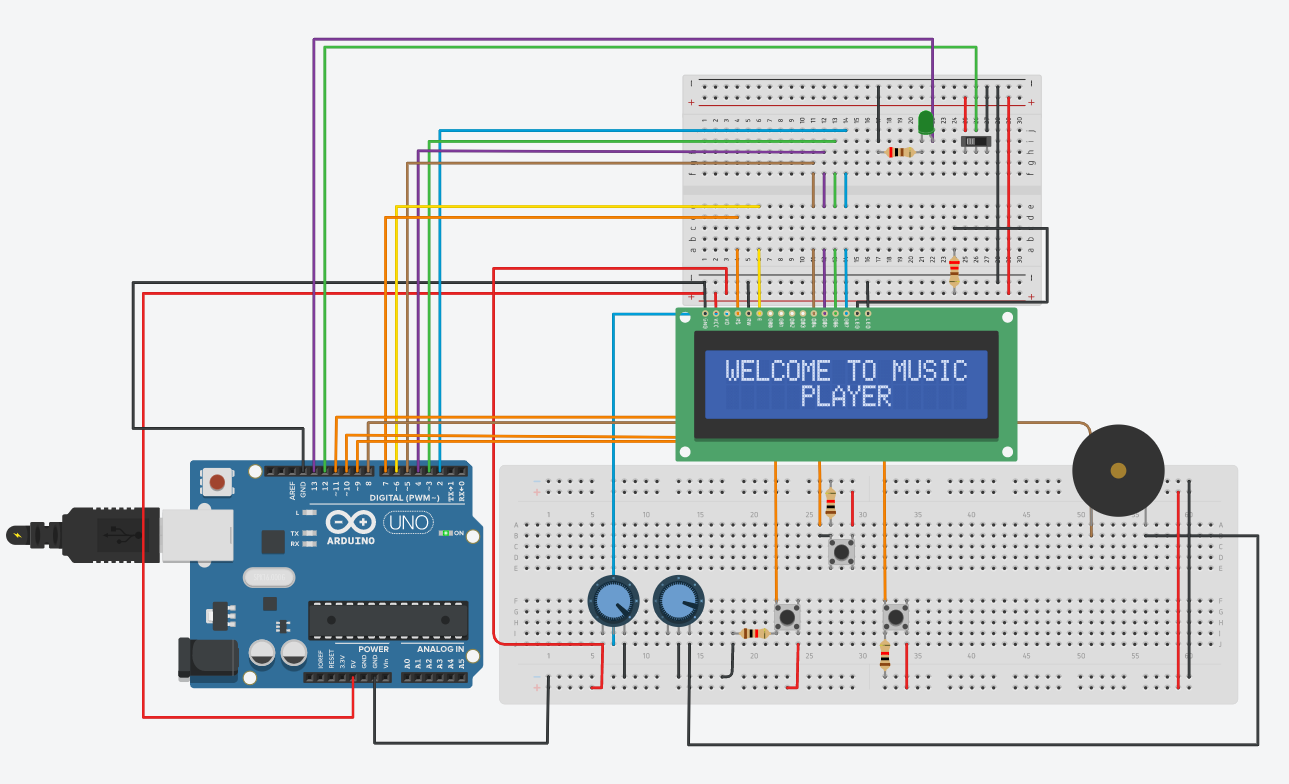
\includegraphics[scale=.45]{Circuit Diagram 1.png}
	\caption{MP3 Player Simulation}
	\label{fig:Circuit 1}
\end{figure}

\begin{figure}[H]
	\centering
	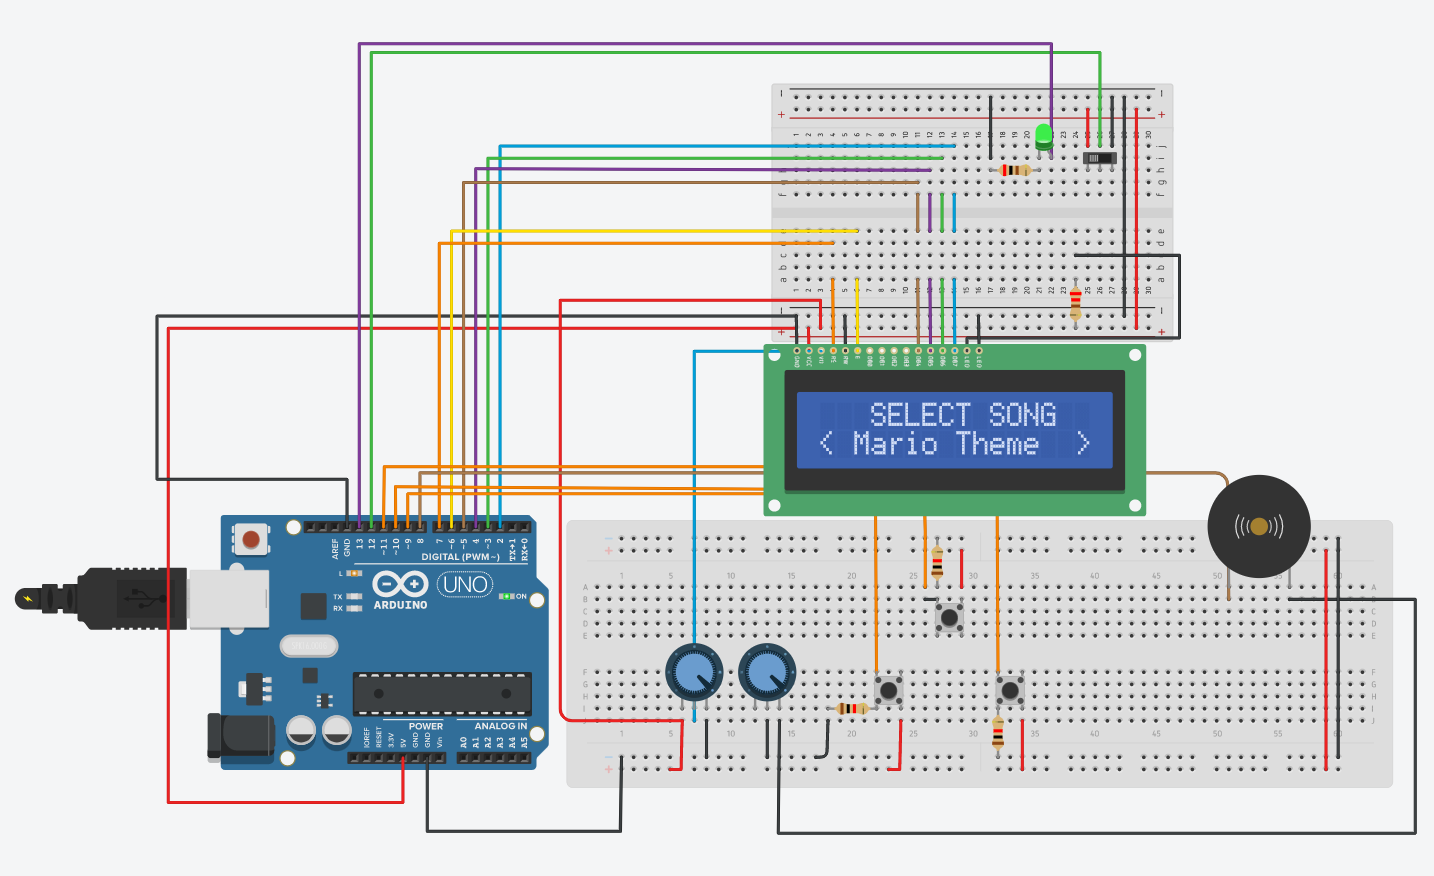
\includegraphics[scale=.40]{Circuit Diagram 2.png}
	\caption{MP3 Player Simulation while working}
	\label{fig:Circuit 2}
\end{figure}

\section{Component List}
The components Used For making the Circuit are listed Below
\begin{table}[H]
	\centering
	\caption{Component List for 8 Bit MP3 Player}
	\vspace{5pt}
	\begin{tabular}{|c|c|c|}
		\hline
		\textbf{Name}       & \textbf{Quantity} & \textbf{Component}  \\ \hline
		{U4}         & 1                 & Arduino Uno R3      \\ \hline
		{U6}         & 1                 & LCD 16 x 2          \\ \hline
		{PIEZO2}     & 1                 & Piezo               \\ \hline
		{D2}         & 1                 & Green LED           \\ \hline
		{S2, S3, S4} & 3                 & Pushbutton          \\ \hline
		{Rpot3}      & 1                 & 5 Ω Potentiometer   \\ \hline
		{Rpot4}      & 1                 & 50 kΩ Potentiometer \\ \hline
		{R3}         & 1                 & 220 Ω Resistor      \\ \hline
		{R1}         & 1                 & 200 Ω Resistor      \\ \hline
		{R4, R2, R5} & 3                 & 1 kΩ Resistor       \\ \hline
		{S1}         & 1                 & Slideswitch         \\ \hline
		
	\end{tabular}
\end{table}

\section{Circuit Explanation and Working}

\subsection{Power}	
Power to the Arduino is given from a standard Li-Ion 3.7V Battery or a 5V Battery or Wall Adapter that outputs 5V 2A.
Power to the LCD Screen and the Buzzer is then supplied from the Arduino.

\begin{figure}[H]
	\centering
	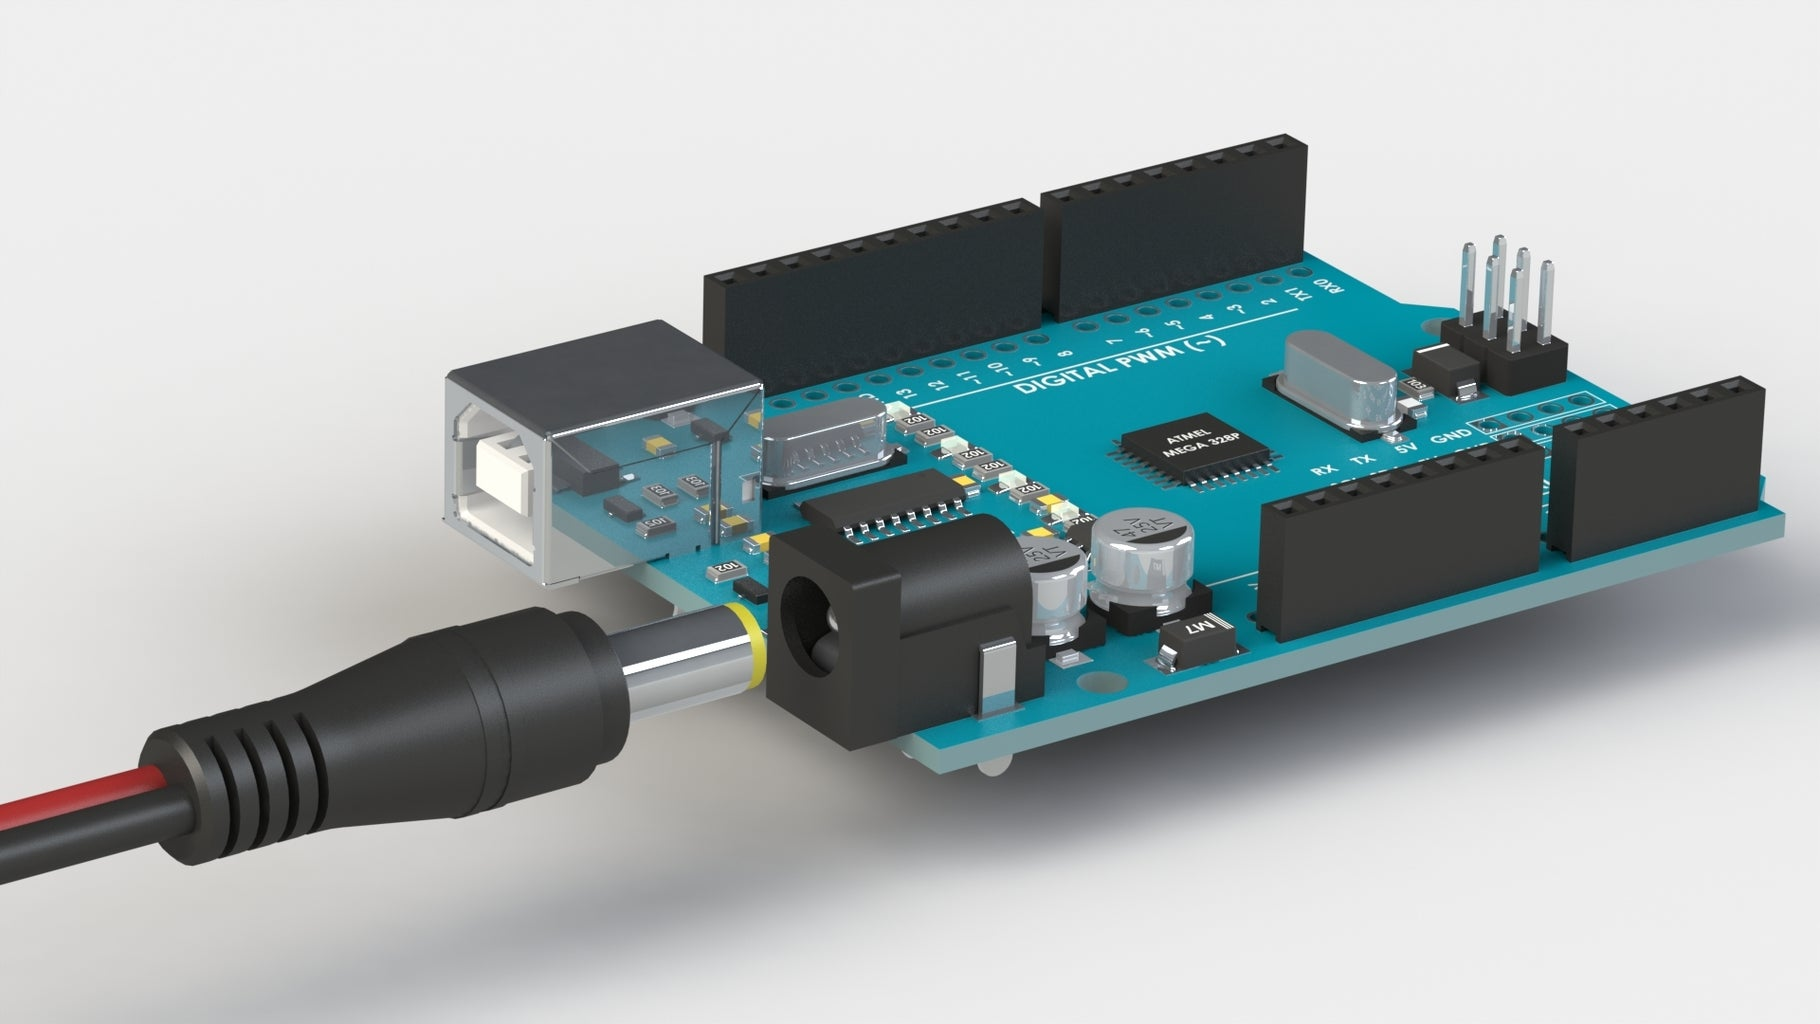
\includegraphics[scale=.25]{arduino.jpg}
	\caption{Power To the Arduino}
	\label{fig:Arduion pic}
\end{figure}

\subsection{Inputs}
Inputs are taken from The Main switch, that controls the Entire working, and push buttons that control the playback. The Volume of the buzzer is controlled by a Potentiometer that simply increases the resistance, and thereby reducing the current passing in the Buzzer, resulting in control of sound. \\

Another Potentiometer controls the Brightness of the LCD Screen in the same way.

\begin{figure}[H]
	\centering
	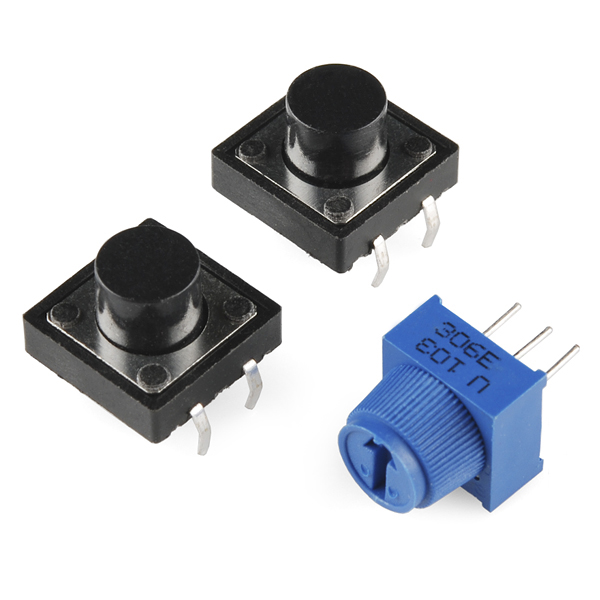
\includegraphics[scale=.8]{push_buttons.jpg}
	\caption{Inputs from Buttons are given to Digital PINS of the Arduino}
	\label{fig:button pic}
\end{figure}

\subsection{Processing}

All of the Processing is done with the Arduino, and the ATMEGA8U2 Chip inside it. If the play button is pressed, it sends a HIGH signal to pin 11 of the Arduino, which is detected, and the Arduino then sends calculated power processed in milliseconds by taking instructions from the code to PIN 8, where the Buzzer is connected. \\

\begin{figure}[H]
	\centering
	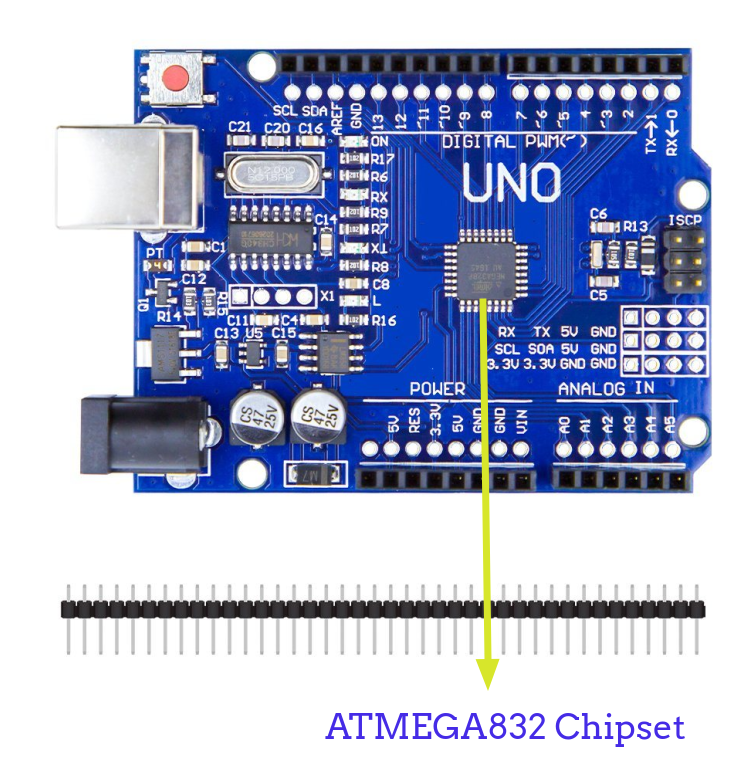
\includegraphics[scale=.45]{chipset.jpg}
	\caption{Chip of the Arduino}
	\label{fig:chipset pic}
\end{figure}

Similarly, When buttons are pressed, they send a voltage to another PIN of the Arduino that is detected, and the song is changed accordingly. 

\subsection{Code}
The Complete code is not shown here due to space restrictions, only the main function names are given to get a crude idea.
 
\begin{lstlisting}
#include <LiquidCrystal.h>
#include <string.h>

// Defining the Basic Notes
#define SA 256
#define RE 280
#define GA 312
#define MA 346
#define PA 384
#define DHA 426
#define NI 480

// Defining the Arduino Input Pins
#define PREV_PIN 10
#define FORWARD_PIN 11
#define PLAY_PIN 9
#define ON_PIN 13
#define SWITCH_PIN 12
#define melodyPin 8

int basic_frequencies[7] = {SA, RE, GA, MA, PA, DHA, NI};
LiquidCrystal lcd(7, 6, 5, 4, 3, 2);

// Declaring Basic Variables and Booleans.
int song = 0, end = 0;
int playing = 0, pause = 1;

// List of Songs
String songs[9] = {
	"Mario Theme",
	"Mario Theme 2",
	"Frequency Sa",
	"Frequency Re",
	"Frequency Ga",
	"Frequency Ma",
	"Frequency Pa",
	"Frequency Dha",
	"Frequency Ni",
};

// Mario main theme melody
int melody[] = {};

// Mario main them tempo
int tempo[] = {};

// Mario Theme 2 melody
int mario_theme_2_melody[] = {};

// Underworld tempo
int mario_theme_2_tempo[] = {};

// Control which notes to play
void sing(int s) {}

// Play those notes. 
void buzz(int targetPin, long frequency, long length) {}

// Main Setup Function
void setup()
{
	// Print WELCOME TO MUSIC PLAYER on the LCD Screen
	// Print First Song after 3 Seconds
	
	// Declare Output PINS
	pinMode(melodyPin, OUTPUT); // buzzer
	pinMode(ON_PIN, OUTPUT);    // LED
	
	// Declare INPUT PINS
	pinMode(SWITCH_PIN, INPUT);  // main switch
	pinMode(PLAY_PIN, INPUT);    // Play/Pause
	pinMode(PREV_PIN, INPUT);    // Previous song
	pinMode(FORWARD_PIN, INPUT); // Next song
}

void loop()
{
	// Check if The Main switch is turned on, only then we do anything.
	if (digitalRead(SWITCH_PIN) == 1)
	{
		// Switch on the LED indicating that we have turned on.
		digitalWrite(ON_PIN, HIGH);
		
		// If user presses forward, change song and show it.
		if (digitalRead(FORWARD_PIN) == 1) {}
		
		// If user presses Previous, change song and show it.
		if (digitalRead(PREV_PIN) == 1) {}
		
		// If user presses play, then play the song
		if ((digitalRead(PLAY_PIN) == 1) && (playing == 0) && (pause = 1)) {}
		end = 0;
	}
	
	// If the main switch is off, then turn of the LED and Print Thank You.
	else if ((digitalRead(SWITCH_PIN) == 0) && (end == 0)){}
}

	
\end{lstlisting}

\subsection{Outputs}
PIN 8 of the Arduino sends Power to the buzzer or alternatively a speaker that will produce the sound at the desired Frequency.

\begin{figure}[H]
	\centering
	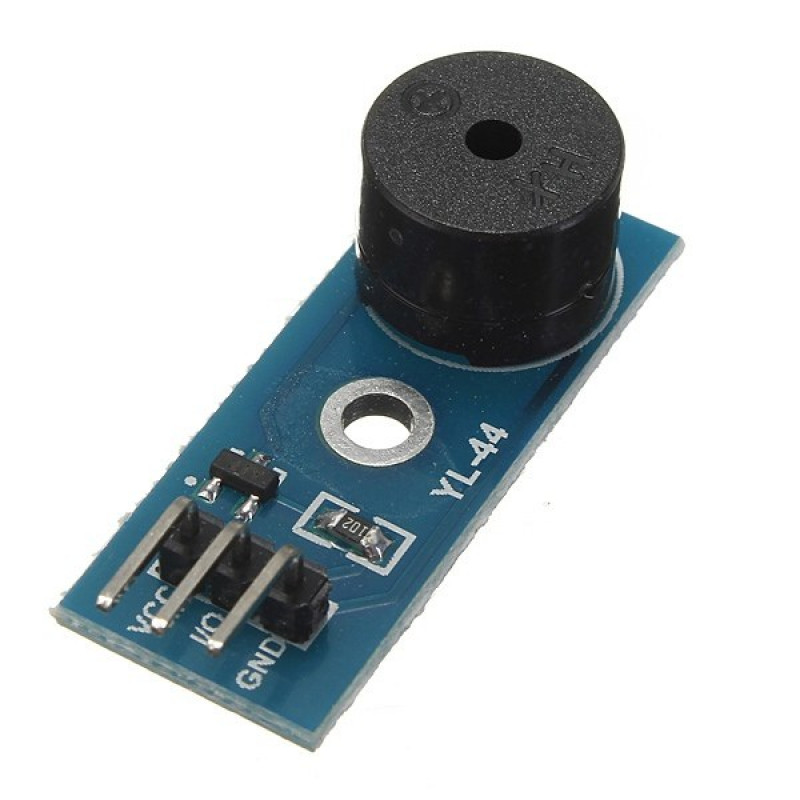
\includegraphics[scale=.2]{buzzer.jpg}
	\caption{The Speaker or Buzzer in User}
	\label{fig:buzzer pic}
\end{figure}

Digital PIN 2 - Digital PIN 7 of the Arduino, along with 5V Power and Ground connects to various inputs of the LCD Screen which then outputs the current song that is being played. 

\begin{figure}[H]
	\centering
	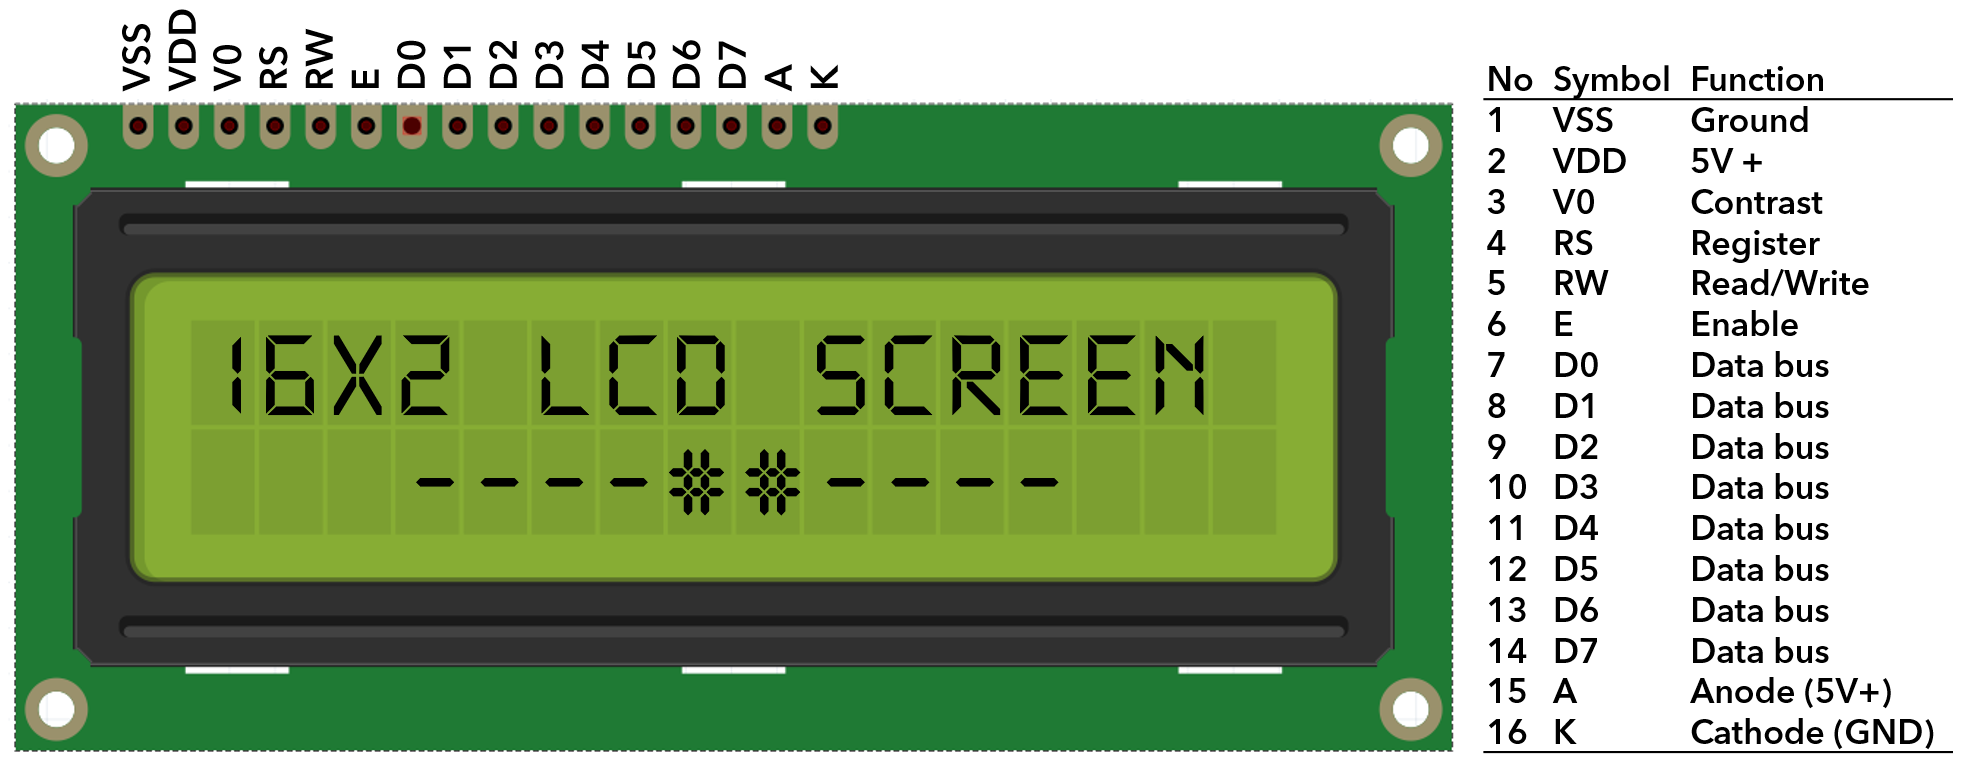
\includegraphics[scale=.45]{LCD.png}
	\caption{16 Pin LCD Screen}
	\label{fig:lcd pic}
\end{figure}


\section{Applications}
\begin{enumerate}
\item An Arduino being far superior than required for a project like this one, would make it impractical to buy and use, but the Chipset, and certain music ICs paired with the same arrangement as in this project can be used to make a good 8-Bit Music Player.
\item The Arduino itself has numerous Applications like: 
\begin{enumerate}
	\item Weighing Machines.
	\item Traffic Light Count Down Timer.
	\item Parking Lot Counter.
	\item Home Automation.
	\item Industrial Automation.
	\item Medical Instrument.
	\item Emergency Light for Railways.
\end{enumerate}

\item The LCD Screen can also be used to display anything from a clock,
a timer, weights, Temperatures, or any needed value, cheaply and easily.
\item More Songs can be programmed and added to then put this into something very small and
portable for a quick, simple and cheap Music Player.

\end{enumerate}


\subsection{Improvements}
\begin{enumerate}
	\item The Expensive Arduino can be replaced with the
	chipset used inside or another Music IC coupled
	with another cheaper Microprocessor IC to reduce
	the cost (while increasing the complications) of the
	Project.

	\item A Better Buzzer can be used for better sound
	Quality
	
	\item A Program can be written that automatically
	converts any song into its 8 Bit code version so it
	becomes easy to add new songs, instead of hard
	coding them into the Aruduino.
	
	\item An External Storage of some sort can be added like
	an SD Card to store Thousands of other Songs.
	
	\item All The components can be put in a small Enclosing
	for increasing Portabitlity.

\end{enumerate}

\section{Conclusion}
\subsection{Learning Experience}
\begin{enumerate}
	\item I got to interact with the Basic LCD Screen, and so now that can be used in many
	other places, which is an important output device.
	\item Exposure to a Microprocessor and working on such a low level of input and output
	gave a better and more open idea about the working of a computer.
	\item 2 Terminal Switches are basic, but 3 terminal switches with a ground pin make use of
	more Electrical concepts which were put to use by actually using them. This
	also forced me to learn the basics of the Potentiometer and its detailed working.
	\item Programming the Basics of Music also made me learn some Music Theory, reading
	some music notes, and an in depth working of a speaker.
\end{enumerate}

\subsection{Conclusion}
A very simple 8-bit Music Player was made, programmed and Built in
Tinkercad successfully. The Working, Programming, and basic functioning of the Arduino, a
Buzzer, an LCD Screen, Switches and Potentiometer was studied and
Applied in detail.
\pagebreak
\begin{thebibliography}{}
	
\bibitem{source 2}
Tinkercad Website for Circuit Design\\
\url{https://www.tinkercad.com/}

\bibitem{some source}
Mario Theme Song on Tinkercad\\
\url{https://www.tinkercad.com/things/26ARFLeA0mg-mario-theme-song}

\bibitem{source 3}
Music Notes for the Mario Theme Song\\
\url{https://www.youtube.com/watch?v=soTO2ywdViA}

\bibitem{source 4}
Working of the Potentiometer\\
\url{https://www.electrical4u.com/potentiometer}

\bibitem{source 5}
Working of the 3 Way Switches\\
\url{https://matthews.sites.wfu.edu/courses/p230/switches/SwitchesTut.html}

\end{thebibliography}

\end{document}